\chapter{Geometric transforms}

\section{Problem statement}

Develop a geometric transform program that will rotate, translate,
and scale an image by specified amounts, using the nearest neighbor
and bilinear interpolation methods, respectively.

\section{Python implementation}

Usage:~\textbf{problem6.py [-h] -i INPUT} \\
       \textbf{(-t TRANSLATE [TRANSLATE ...] | -r ROTATE | -s SCALE)}
       \textbf{(--nearest | --bilinear) [--truncate] [--debug]}

Use \textbf{python problem6.py -h} to see the help.

\pagebreak

%\begin{figure}[!htb]\centering
    %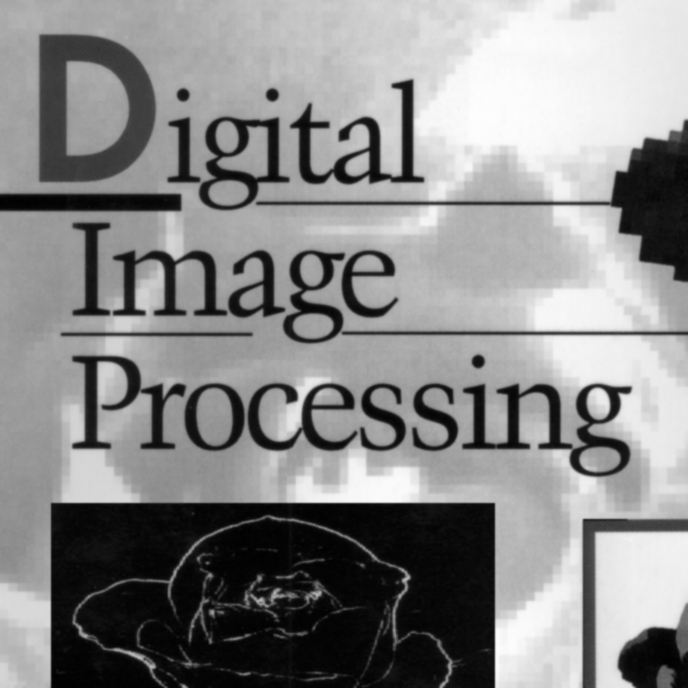
\includegraphics[width=0.6\linewidth]{./images/6/original.jpg}
    %\caption{\small{Original image}}
%\end{figure}

\pagebreak

\section{Translation}

%\begin{minipage}{\textwidth}
%\textbf{python problem5.py --inv book\_cover.jpg} \\
%\textbf{python problem5.py --noise -s 650 --inv book\_cover.jpg}
%\end{minipage}

%\begin{figure}[!htb]\centering
    %\begin{minipage}{0.45\textwidth}
        %\frame{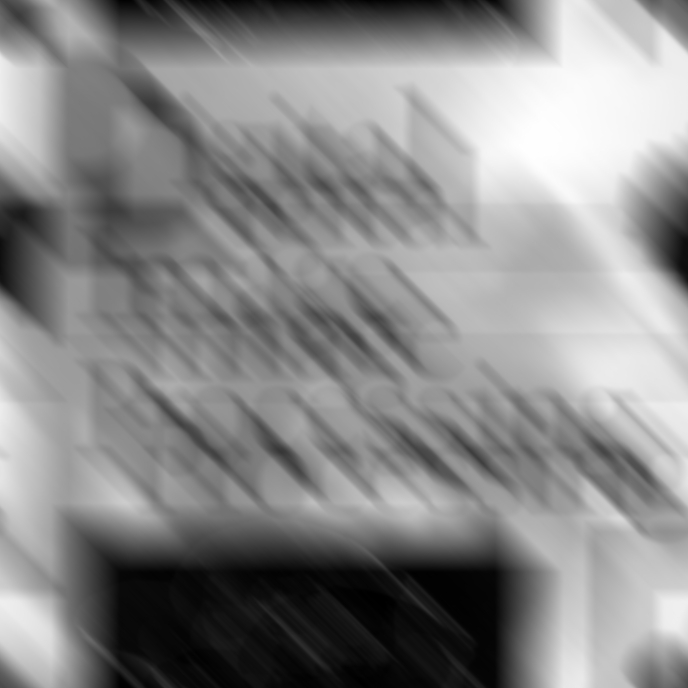
\includegraphics[width=\linewidth]{./images/5/blurred.jpg}}
        %\caption{\small{Blurred image}}
    %\end{minipage}
    %\begin{minipage}{0.45\textwidth}
        %\frame{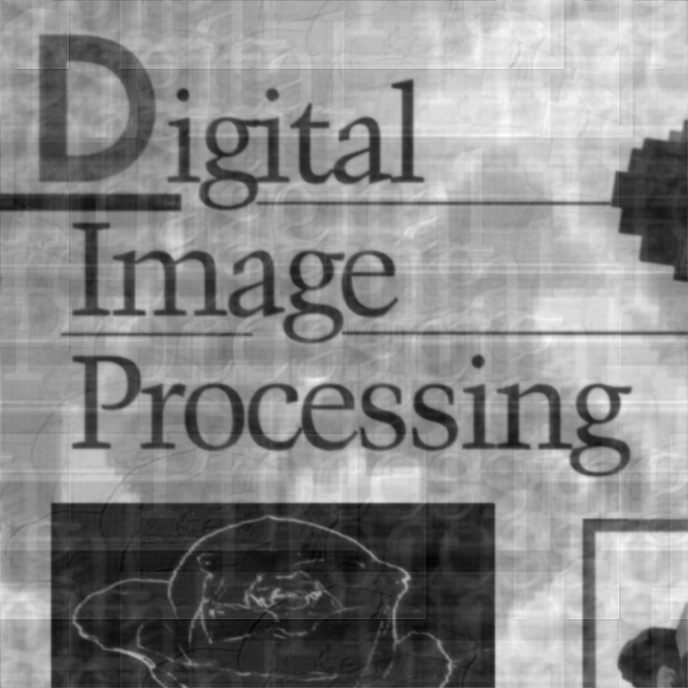
\includegraphics[width=\linewidth]{./images/5/inv_blurred.jpg}}
        %\caption{\small{Inverse blurred image}}\label{diagram:inv_blurred}
    %\end{minipage}
%\end{figure}

%\begin{figure}[!htb]\centering
    %\begin{minipage}{0.45\textwidth}
        %\frame{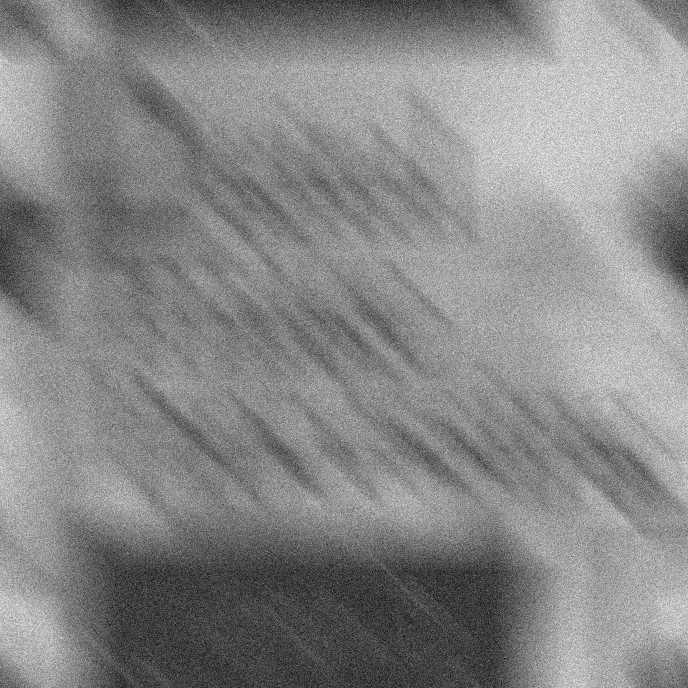
\includegraphics[width=\linewidth]{./images/5/blurred_noise.jpg}}
        %\caption{\small{Blur + noise}}
    %\end{minipage}
    %\begin{minipage}{0.45\textwidth}
    %\frame{
\includegraphics[width=\linewidth]{./images/5/inv_blurred_noise.jpg}}
    %\caption{\small{Inverse 'blur + noise'}}\label{diagram:inv_blurred_noise}
    %\end{minipage}
%\end{figure}
